\section*{Analyse} % (fold)
\label{sec:analyse}
Das Resultat ist in Abbildung \ref{pic:sim} dargestellt. Die dunkel gestrichelte Linie ist repräsentiert die neunte Dezille bezogen auf die durch die Farbe repräsentierte Anzahl an Köchen. Die zuvor definierte Frage \textit{Wie viele Köche müssen beschäftigt werden damit mindestens 90\% aller Gäste, 10min nach ihrer Bestellung, ihre Welfencreme bekommen?} lässt sich mit \textit{es werden drei Köche benötigt} beantworten.
\paragraph{Beobachtungen}
Aus betriebswirtschaftlicher Sicht ist es evtl. besser sich nur für zwei Köche zu entscheiden, weil der zeitliche Nachteil gegenüber drei Köche nicht groß ist (ungefähr 20 sec. bei der neunten Dezille). Eine weitere interessante Beobachtung ist, dass die größte zeitliche Verbesserung bei dem Sprung von einem auf zwei Köche zu verzeichnen ist. Der Median sinkt von 866,9 auf 575,5 Sekunden. Betrachtet man dazu im Vergleich die Beschleunigung beim Einsatz von sechs, statt vier Köche, hat man nur eine Verbesserung von ca. zwölf Sekunden im Median.
Dieses Verhalten kann man auch in der IT, beim Einsatz von mehreren Prozessoren beobachten. Sofern die Anwendung nicht auf mehr Prozessoren ausgelegt ist, ist die Performanceverbesserung durch den Einsatz von mehr Prozessoren nur sehr marginal. \\

Eine weitere interessante Beobachtung ist, dass mit steigender Zahl Köche die Verteilung schmaler wird (geringere Standardabweichung). Dieser Trend wird lediglich von der Messung mit 4 Köchen gebrochen. Dieser Ausreiße lässt sich unter Umständen mit der geringen Samplesize des Experiments erklären. Intuitive lässt sich dieses Verhalten gut dadurch nachvollziehen, dass mit steigender Anzahl Köche die Wahrscheinlichkeit steigt das eine Tätigkeit die erledigt werden kann auch sofort aufgenommen wird. Dieser Trend wird spätestens dann verschwinden wenn die Anzahl der Köche größer ist als die Anzahl der Tätigkeiten die maximal gleichzeitig geschehen können. Die maximale Anzahl an Tätigkeiten die gleichzeitig geschehen können ist in unserem Petrinetz ist 5. Es existiert nur ein Szenario: ein Koch schlägt die Weinsoße schaumig und erhitzt sie und 4 Köche füllen jeweils eine Portion Vanillecreme ab. Mit dieser Information lässt sich somit auch gut die sehr geringe Verbesserung von 4 auf 6 Köche erklären, weiter lässt sich folgern das 5 Köche genau so schnell arbeiten können wie 6 Köche. Da bei 6 Köchen ein Koch immer nichts zu tun hat.\\

Der Vergleich mit realen Bedingungen in einem Gastronomiebetrieb ist allerdings nur bedingt möglich da einerseits in einer Küche viele andere Aufgaben erledigt werden, wie zum Beispiel Putzen, und das Kochen einer Speise häufig meist nicht von so vielen Köchen gemacht wird. In dem konkreten Beispiel für die Erstellung von Welfencreme würde in einem Restaurant höchstwahrscheinlich eine sehr große Menge von einem Koch vorbereitet werden um dann während der Hauptgeschäftszeit lediglich aus der Kühlung geholt zu werden.

\begin{figure}[ht]
  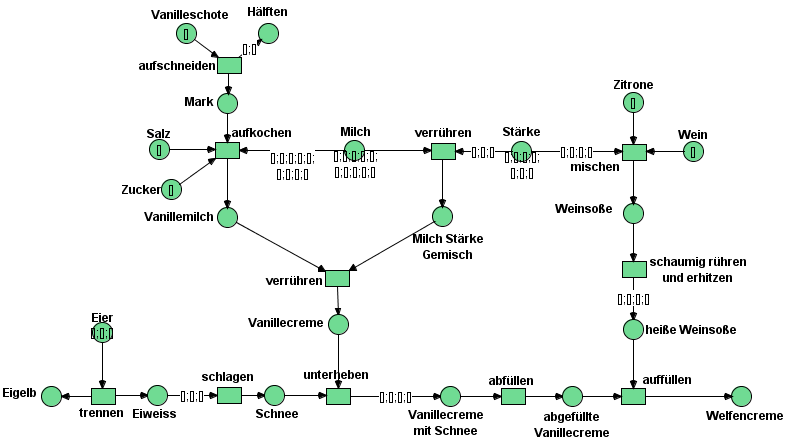
\includegraphics[width=1\textwidth]{pics/sim.png}
  \caption{Histogramm: Die Simulation des Petrinetzes mit verschiedener Anzahl Köchen, gepunktet der korrespondierende Median, dunkel gestrichelt 9. Dezille}
  \label{pic:sim}
\end{figure}


% Wie haben wir die Daten gewonnen ?
% Autohotkey ...
% java -jar loader.jar gui > data.txt

%Denk an die Fragestellung die ich aufgestellt habe und sag in wie weit die Ergebnisse auf eine reale Arbeitsumgebung anwendbar sind (nur bedingt ...)

% 9. Dezille heißt, dass 90% der Werte unterhalb dieses Wertes liegen und 10% drüber -> Fragestellung
